\section{Teilchen in Materie}
\subsection{Bethe-Bloch}
Geladene Teilchen die sich durch Materie bewegen verlieren durch Interaktionen mit den Atomen an Energie. Diese Interaktionen umfassen Bremsstrahlung bei hohen Energien, Ionisation bei mittleren Energien und Anregung von Atomen bei geringen Energien. Der Energieverlust in Abhängigkeit von der Energie des Teilchens ist in Abb. \ref{fig:bethe} dargestellt. Für schwere geladene Teilchen, wie z.B. das Muon wird der Energieverlust durch Ionisation durch die Bethe-Bloch Formel beschrieben\cite{Passage_through_matter}.
\begin{align}
- \left<\frac{dE}{dx}\right> =  K\cdot \frac{Z}{A}\frac{z^2}{\beta^2} \cdot \left[ \frac12\ln \left(\frac{2m_ec^2\cdot\beta^2\cdot\gamma^2 \cdot T_{max}}{I^2}\right) - \beta^2 - \frac{\delta(\beta\gamma)}{2}\right] \label{eq:bethe}
\end{align} 
Diese Formel hängt lediglich von der Ladung $z$ und der relativistischen Geschwindigkeit $\beta$ des Teilchens und dem Material $K$ ab. Sie hängt explizit nicht von der Masse des Teilchens ab. Sie gibt den mittleren Energieverlust pro Strecke an. 
\begin{figure}
\centering
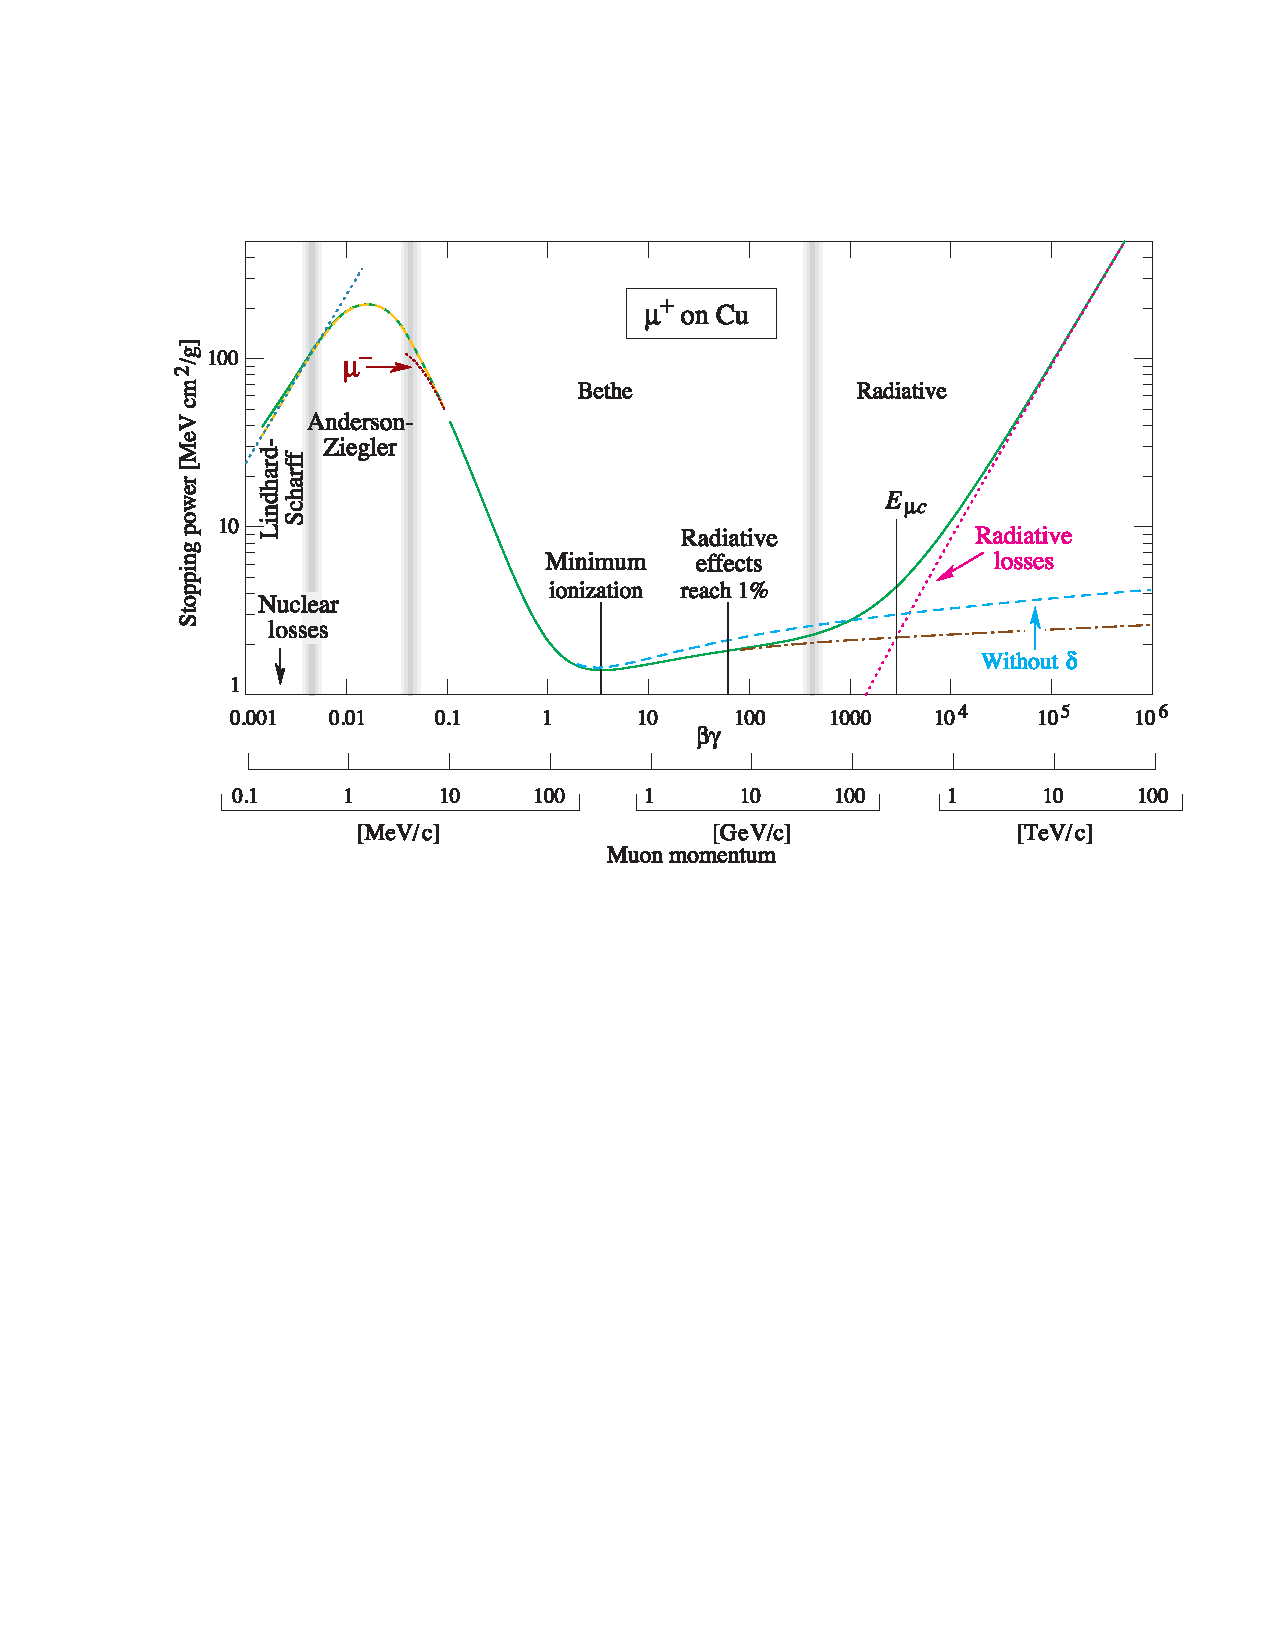
\includegraphics[scale=0.7]{./input/bethe.pdf}\caption{Energieverlust pro Strecke (Stopping power) aufgetragen gegen den Impuls eines Muons. Der Verlust durch Ionisation findet in einem Bereich von 10~Mev und 100~GeV statt\cite{Passage_through_matter}.}\label{fig:bethe}
\end{figure}
Um diesen Mittelwert ist der Energieverlust nach der Landau-Verteilung verteilt.
\begin{figure}
\centering
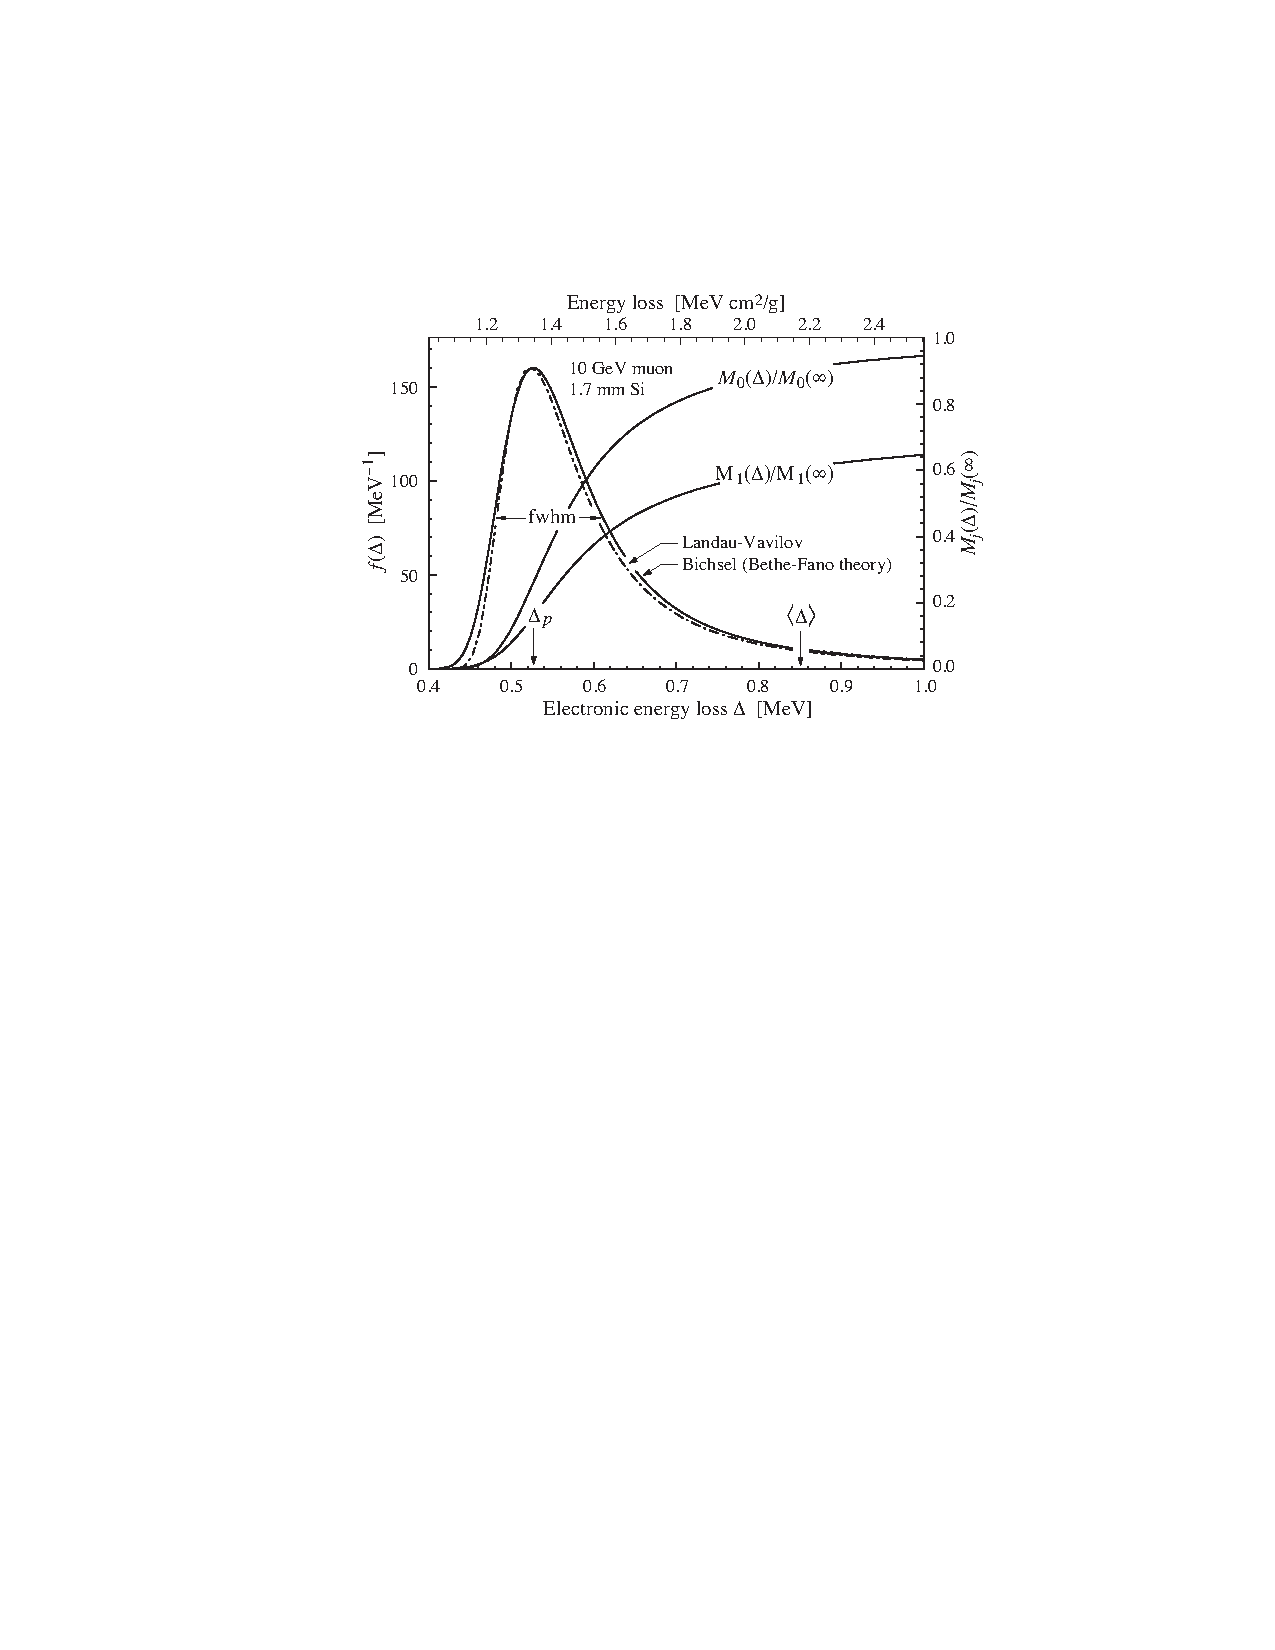
\includegraphics[]{./input/landau.pdf}\caption{Landau-Verteilung des nach Bethe-Bloch berechneten Energieverlusts.\cite{Passage_through_matter}}\label{fig:landau}
\end{figure}
\subsection{Elektronen und Photonen}
Photonen und Elektronen verlieren ihre Energie in Materie hauptsächlich durch Bremsstrahlung (Elektronen), und Paarerzeugung (Photonen). Weil ein Elektron durch Bremsstrahlung Photonen aussendet und ein Photon durch Paarerzeugung Elektronen erzeugt sind beide Vorgänge eng miteinander verbunden. Eine Materialkonstante, die eine wichtige Rolle spielt ist die Strahlungslänge $X_0$. Sie entspricht der Länge nachdem ein Elektron in Materie alles bis auf $1/e$ seiner Energie abgegeben hat. Gleichzeitig ist es $7/9$ der mittleren freien Weglänge eines Photons in diesem Material. Die aufeinander folgende Bremsstrahlung und Paarerzeugung von Photonen und Elektronen führt zu einer Teilchenkaskade.

\section{Gas-Detektoren}
\subsection{Lawinen-Bildung}
Gas-Detektoren sind Ionisationskammern. Sie bestehen im Allgemeinen aus einer Anode und einer Kathode zwischen denen sich ein Gas als Ionisationsmedium befindet. Trifft ein ionisierendes Teilchen in die Kammer, so schlägt es Elektronen aus den Gasmolekülen heraus. Diese Elektronen werden durch die Spannung zwischen Anode und Kathode beschleunigt, sodass sie selbst wieder genug kinetische Energie haben um selbst Moleküle zu ionisieren. Ein einfallendes Teilchen produziert auf diese Weise eine Elektronen-Lawine, die als messbarer Strom zwischen Anode und Kathode nachgewiesen werden kann. In Abhängigkeit von der angelegten Spannung ist das Signal entweder proportional zu der durch das ursprünglich einfallende Teilchen verursachten Ionisation, oder für jedes Teilchen gleich. Der letztere Fall tritt zum Beispiel beim Geiger-Müller-Zählrohr auf, bei dem lediglich gemessen wird ob ein ionisierendes Teilchen im Zählrohr aufgetroffen ist oder nicht. Für die Teilchenpyhsik sind vor allem Detektoren von Nutzen, die ein zur Ionisation proportionales Signal liefern, da in diesem Fall zwischen Teilchen unterschieden werden kann.
\subsection{Die Multi-Wire-Proportional-Chamber(MWPC)}
Die MWPC ist eine Ionisationskammer bestehend aus vielen einzelnen Anodendrähten und Kathodenplatten die parallel zur Ebene der Drähte angeordnet sind(siehe Abb. \ref{fig:MWPC}). Durch die Verwendung mehrerer Anodendrähte ist es möglich den Einschlagsort des Teilchens in der Achse senkrecht zu den Anodendrähten zu bestimmen. Verwendet man mehrere Ebenen so lassen sich auch zwei- und dreidimensionale Messungen durchführen.
\begin{figure}
\centering
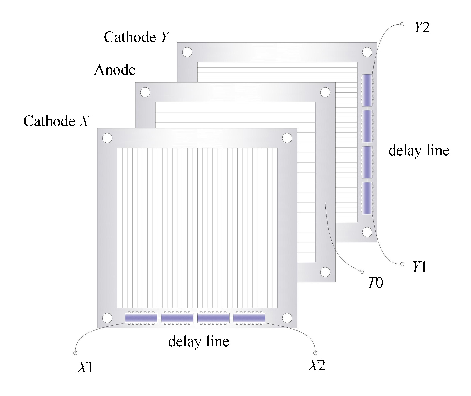
\includegraphics[]{./input/MWPC.eps}\caption{Schematische Darstellung einer MWPC\cite{Tang:2013daa}.}\label{fig:MWPC}
\end{figure}
\subsection{Driftkammer}
Die Driftkammer ist eine Ionisationskammer in der ein sehr homogenes elektrisches Feld herrscht. Die durch Ionisation freiwerdenden Elektronen haben eine nahezu konstante Driftgeschwindigkeit zur Anode, und werden erst in unmittelbarer Nähe der Anode stark beschleunigt um eine Lawinenbildung zu ermöglichen. Ist der Einschlagszeitpunkt des Teilchens bekannt, so ist es möglich aus der Zeitdifferenz zwischen Zeitpunkt des Auftreffens und Signal den Abstand des Teilchens von der Anode zu berechnen. Auf diese Weise ist eine größere Ortsauflösung bei gleichzeitig weniger Materialkosten zu erzeugen.
Eine häufig benutzte Variante der Driftkammer ist das Driftröhrchen (Drifttube). Drifttubes finden z.B. im \atlas-Detektor Anwendung, wo sie zur Detektion von Myonen eingesetzt werden. Im \atlas werden sie dabei leicht versetzt geschichtet eingesetzt, sodass eine gute Auflösung in den beiden Achsen senkrecht zu den Drifttubes möglich wird. Den Auftreffort des Teilchen in der Achse parallel zu den Drifttubes kann man über die Stärke des Signals an beiden Enden des Drifttubes bestimmen. Die Ionisationslawine fließt in beide Richtungen des Anodendrahtes ab, die Stärke des Signals jedoch hängt jedoch von der zurückgelegten Strecke ab. Aus dem Verhältnis der Signale lässt sich berechnen an welcher Stelle des Drahtes die Ionisation stattgefunden hat.
\subsection{Time-Projection-Chamber (TPC)}
Die TPC funktioniert ähnlich wie die Driftkammer mit dem Unterschied, dass in der TPC die Anode eine Fläche ist, die aufgeteilt in Anodensegmente ist. In jedem der Segmente lässt sich unabhängig von benachbarten Segmenten ein Strom messen. Durchquert ein Teilchen die TPC so hinterlässt es eine Spur aus Ionen und Elektronen. Die Elektronen driften nun zur Anode hin, aus den Zeitpunkten zu denen die Elektronen auf die Anodensegmente auftreffen lässt sich nun die gesamte Bahn des Teilchens rekonstruieren. Der Abstand der Teilchenbahn zur Anode wird also auf die Zeit die Elektronen zu Anode brauchen projiziert.
\section{Teilchen Identifikation}
Teilchen können auf verschiedene Weisen identifiziert werden. Am einfachsten ist die Identifikation durch ihre Interaktion mit dem Detektor. Geladene Teilchen hinterlassen eine Spur im Spurdetektor, und erzeugen einen Schauer im elektromagnetischen(EM) Kalorimeter. Anhand der Krümmung der Spur kann die Ladung und der Impuls des Teilchens bestimmt werden. Auf diese Weise werden Elektronen detektiert. Photonen bilden keine sichtbare Spur im Spurdetektor, erzeugen jedoch einen Schauer im elektromagnetischen Kalorimeter, können also auf diese Weise identifiziert werden. Geladene Hadronen wie z.B. das $\pi^+$-Meson, hinterlassen sowohl eine Spur im Spurdetektor als auch einige Hits im EM Kalorimeter. Zusätzlich erzeugen sie einen Schauer im hadronischen Kalorimeter. Neutrale Hadronen wie das Neutron hinterlassen keine Spur im Spurdetektor, und sind auch im EM Kalorimeter nicht messbar. Allerdings erzeugen sie einen Schauer im hadronischen Kalorimeter. Somit sind sie auf diese Weise nachweisbar. Ein Problem stellt das Myon dar, was trotz Ladung, nicht durch die Kalorimeter gestoppt wird. Myonen werden durch spezielle Myonenkammern detektiert, die die äußersten Bestandteile eines Detektors bilden. Bei dem Myonenkammern handelt es sich um Ionisationskammern. Beim \atlas-Detektor sind dies Drifttubes. Außer den Myonen hinterlassen keine anderen Teilchen Spuren in den Myonkammern, da sie bereits in den Kalorimetern gestoppt wurden.
Neutrinos können nicht detektiert werden, da sie nur schwach wechselwirken. Deswegen können Neutrinos nur aus der transversalen Impulserhaltung rekonstuiert werden wobei deren Energie als \emph{missing transverse energy} \MET bezeichnet wird.

Andere Möglichkeiten Teilchen zu identifizieren umfassen den Energieverlust eines Teilchen ins Materie, wobei die Ladung des Teilchens aus der Bethe-Bloch-Formel (\ref{eq:bethe}) bestimmt werden kann, Time-of-Flight Detektoren, die die Zeit messen die ein Teilchen braucht um sich von einem Interaktionspunkt zu einem zweiten zu bewegen, und Cherenkov-Detektoren. 

\section{Cherenkov Detektoren}
text
\section{Halbleiter Detektoren}
\subsection{Halbleiter}
\subsection{Strahlungsschäden}
\subsection{Signalerzeugung}
\subsection{Silizium Detektor}
text
\section{Kalorimeter}
\subsection{Elektromagnetische Schauer}
\subsection{Hadronische Schauer}
\subsection{Sampling und homogene Kalorimeter}
\subsection{Energieauflösung}
text
